\documentclass[11pt]{article}

\usepackage[T1]{fontenc}
\usepackage[utf8]{inputenc}
\usepackage{amsmath}
\usepackage{amssymb}
\usepackage[margin=1in]{geometry}
\usepackage[numbers,sort&compress]{natbib}
\usepackage[hidelinks]{hyperref}
\usepackage{graphicx}
\usepackage{booktabs}
\usepackage{array}
\usepackage{tikz}
\usetikzlibrary{arrows.meta, positioning}
\bibliographystyle{unsrtnat}

\begin{document}

\begin{titlepage}
\centering
\thispagestyle{empty}

\vspace*{1.5cm}
{\large National Institute of Business Management -- Kandy Innovation Centre \par}
\vspace{0.3cm}
{\normalsize BSc (Hons) in Computer Science -- Artificial Intelligence \par}

\vspace{2.5cm}
{\Large \bfseries Machine Learning and Related Applications \par}
\vspace{0.4cm}
{\large Assignment, Phase 1 \par}
\vspace{0.2cm}
{\large \itshape Conceptual Mapping (Deconstruction) \par}

\vspace{2.5cm}
\rule{\linewidth}{0.6pt} \par
\vspace{0.4cm}
{\normalsize A deconstruction and reconstruction of the following paper: \par}
\vspace{0.5cm}
{\large \bfseries Bioacoustic Classification of Avian Calls from Raw Sound Waveforms with an Open Source Deep Learning Architecture \par}
\vspace{0.4cm}
{\normalsize Bravo Sanchez, F.~J., Hossain, M.~R., English, N.~B. and Moore, S.~T. (2021) \par}
{\normalsize \textit{Scientific Reports}, 11, 15733 \par}
\vspace{0.4cm}
\rule{\linewidth}{0.6pt} \par

\vfill

{\large \bfseries M.A.S.I. Malimbada \par}
\vspace{0.3cm}
{\normalsize Student ID: KIC-BSCCSAI-251P-014 \par}
\vspace{0.2cm}
{\normalsize \href{mailto:KIC-BSCCSAI-251P-014@student.nibm.lk}{KIC-BSCCSAI-251P-014@student.nibm.lk} \par}

\vspace{1.5cm}
{\normalsize \today \par}

\end{titlepage}

\setcounter{page}{1}

\section{Problem Formulation}

\subsection{The underlying domain problem}

This research tackles the area of passive acoustic monitoring, which is used to detect wildlife species by using autonomous recorders left in the field \citep{bravosanchez2021}. Passive acoustic monitoring is highly useful because it removes humans from the field, making it possible to cover large areas and monitor species that try to stay away from humans \citep{digby2013, darras2019}. However, a big problem that comes with passive acoustic monitoring is its volume. PAM produces large amounts of output, a volume that is difficult for a team of humans to review by themselves \citep{campos2019}.

Bio-acoustic species classifiers are used to fix this problem, but they are built on top of a fixed preprocessing pipeline. A raw audio waveform is converted into a spectrogram, then often into a Mel spectrogram, and sometimes further into Mel-frequency cepstral coefficients (MFCCs), and only this transformed, lower-dimensional representation is ever shown to a classifier \cite{stowellplumbley2014}, as cited in \cite{bravosanchez2021}. The main issue is that these transforms were built around human hearing, not any other species' hearing. So they can compress away acoustic detail that means nothing to a human ear but that a given species' calls may actually depend on, and there is no established way to know in advance which transform, or how much compression, is safe for a given species or task \cite{bravosanchez2021}.

Another main issue is that, when audio is preprocessed based on one species, it might not transfer to another species. It is known that feature extraction performance in bioacoustic tasks can vary based on species \citep{bravosanchez2021}. This means that no single spectrogram or Mel setup exists which generalises across species with different call structures.

To fix these problems, the paper skips the preprocessing steps altogether, making a neural network learn from the raw waveform instead. Prior to this paper, this method had rarely been attempted in bioacoustics, because the high dimensionality of audio makes it impractical, requiring more labelled data than most bioacoustic datasets can provide \citep{bravosanchez2021}.

\subsection{Formal statement of the machine learning problem}

This is a supervised, closed set, multi class audio classification problem, where the input is frame level while the label is event level. Let $x \in \mathbb{R}^{L}$ be a single frame, a fixed length chunk of $L$ raw amplitude samples drawn from a recording sampled at 44.1 kHz with 32 bit depth \citep{bravosanchez2021}. Let $\mathcal{Y} = \{1, \dots, K\}$ be a discrete label set representing species and, for birds, call type. $K$ is not one fixed number for the whole paper, because the experiment is actually repeated three separate times at three different label granularities: all 87 classes (bird species crossed with call type, plus the insect and amphibian classes), the 77 bird-only classes (the same call-type split but with the insect and amphibian rows dropped), and the 51 bird species (where the call, song, and drum rows for one species are merged back into a single label). So $K$ changes depending on which of these three runs is being talked about, and results from one value of $K$ are never directly comparable to results from another value of $K$, since the underlying classification task is a different one each time.

SincNet defines the model as a parametric function

\begin{equation}
f_\theta : \mathbb{R}^{L} \to \Delta^{K-1}
\end{equation}

When a frame $x$ is fed in, it returns a posterior $p_\theta(y \mid x)$, a set of probabilities over the $K$ classes that always add up to one, produced by a final LogSoftmax layer \cite{bravosanchez2021}, citing the architecture from \cite{ravanelli2018}. In training, given a set of frames and labels $\mathcal{D} = \{(x_i, y_i)\}_{i=1}^{N}$, the parameters $\theta$ are optimised to minimise the loss across the training set, which is defined in the equation below.

\begin{equation}
\theta^{*} = \arg\min_{\theta} \; -\frac{1}{N}\sum_{i=1}^{N} \log p_\theta(y_i \mid x_i)
\end{equation}

In this methodology, the model cuts each event into a stack of overlapping frames, $\{x_{e,1}, \dots, x_{e,M_e}\}$, where there are more of them for longer events and fewer of them for shorter events. Even though the events themselves can range from roughly 30 ms to over 4.5 s, this ensures that what is being input to the model is always the same size.

The exact way that one frame is cut out of an event is also worth spelling out, because it is not the same rule every time. If the labelled event is longer than the frame length, the frame is placed at a random position that is guaranteed to sit fully inside the labelled event, so every sample the model sees for that draw genuinely belongs to the tagged call. But some tagged events, a small number, are actually shorter than the frame length itself, and for those the rule flips: the frame is instead placed at a random position that is guaranteed to fully contain the short event somewhere inside it, meaning the model also sees a bit of whatever comes immediately before and after the call. This second case only happens for a tiny fraction of the events in this dataset (worked out directly from the annotation files for this assignment, well under one percent, once the frame length used in the tuned runs is applied), but it still matters conceptually, because it means the model is not always being shown ``pure call'', sometimes it is being shown ``call plus a small amount of context'', and the training code does not tell the model which situation it is in.

To turn the predictions of each sliced frame into one prediction, the model averages what it said about every frame belonging to that event, then picks the class that scored highest on average, which is shown in the equation below.

\begin{equation}
\bar{p}(y \mid e) = \frac{1}{M_e}\sum_{m=1}^{M_e} p_\theta(y \mid x_{e,m}), \qquad \hat{y}_e = \arg\max_{y \in \mathcal{Y}} \; \bar{p}(y \mid e)
\end{equation}

Here, every frame in the group is asked to match the label correctly. Therefore, the model is not trained to answer ``which species produced this whole event'', but to answer ``which class does this one short slice resemble''. The final answer $\hat{y}_e$ is only correct if the majority of predictions correctly predict the class.

\subsection{The statistical shape of the dataset}
\label{sec:stats}

Since the raw wav files and the temporal-annotation CSVs that this dataset is built from are both bundled with this project, it is possible to actually check the statistical claims above directly, instead of just repeating what the paper says about them, and a proper conceptual mapping of the problem probably should not skip this step, since the shape of the input distribution is a big part of why the architecture in Section 2 looks the way it does.

Parsing every annotation file that ships with the 687 training recordings gives 5{,}775 individually tagged rows, spread across 569 files (105 more files have an annotation file that is present but genuinely empty, meaning a human reviewed the recording and tagged nothing, and a further 13 files have no annotation record at all). Once the small number of \texttt{Unknown} and \texttt{Human} tags are dropped, the same way the paper's own pipeline drops them, this comes to 5{,}481 usable tagged rows, which lines up closely with the 5{,}478 figure quoted in the paper once the three sub-10~ms events mentioned in the paper's own methods section are also removed.

\begin{figure}[h]
\centering
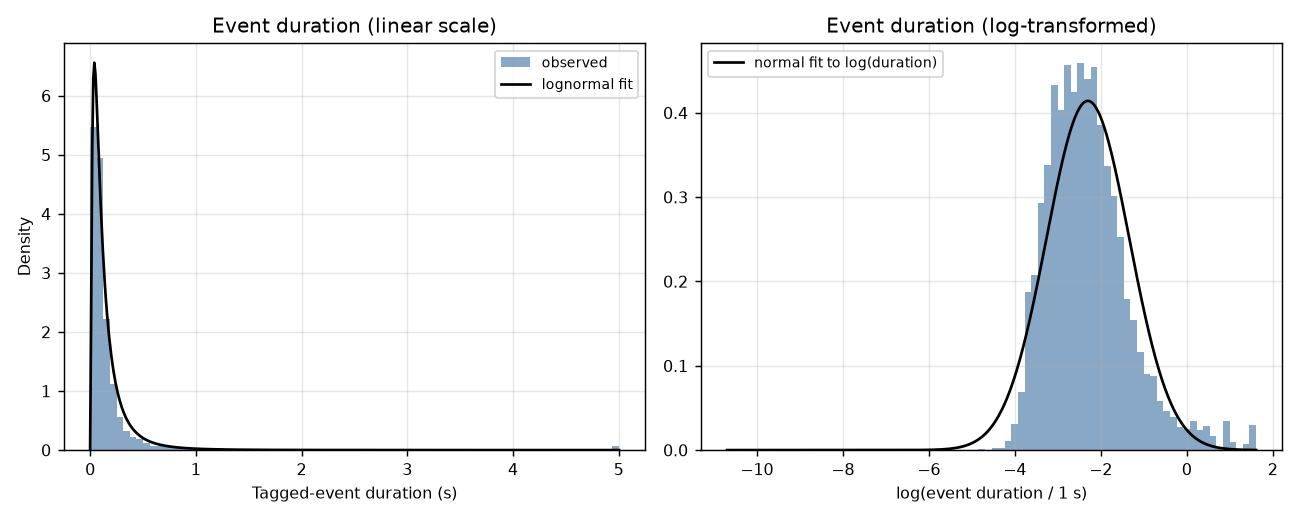
\includegraphics[width=0.72\textwidth]{figures/02_event_duration_distribution.png}
\caption{Duration of the 5{,}775 tagged events, computed directly from the annotation files. Mean 195~ms, median 90~ms, std 455~ms, skewness 7.29.}
\label{fig:eventdur}
\end{figure}

Figure~\ref{fig:eventdur} shows why the window-length decision in Section 2.3 is not really optional. Event duration is very far from being symmetric around its mean: the mean is 195~ms, but the median is only 90~ms, and the distribution has a skewness of about 7.3, which means a small number of very long songs (insect songs especially, some lasting the full 5 seconds) are dragging the mean well above where the bulk of the data actually sits. Fitting a few standard distribution families to this by maximum likelihood and ranking them by AIC picks out the lognormal family by a wide margin over Normal, Gamma, Weibull, or Exponential, with a fitted scale parameter around 0.10~s, matching the empirical median almost exactly. This is roughly what would be expected if a call's length is the product of several smaller, roughly independent multiplicative factors, such as how many syllables it has and how long each syllable and pause lasts, since products of positive random variables tend towards a lognormal shape. Once the frame length used in the tuned runs (16 or 18~ms depending on the class set) is checked against this distribution, only about 0.24 percent of all tagged events turn out to be shorter than it, which is the concrete number behind the ``padding'' case described in Section 1.2.

\begin{figure}[h]
\centering
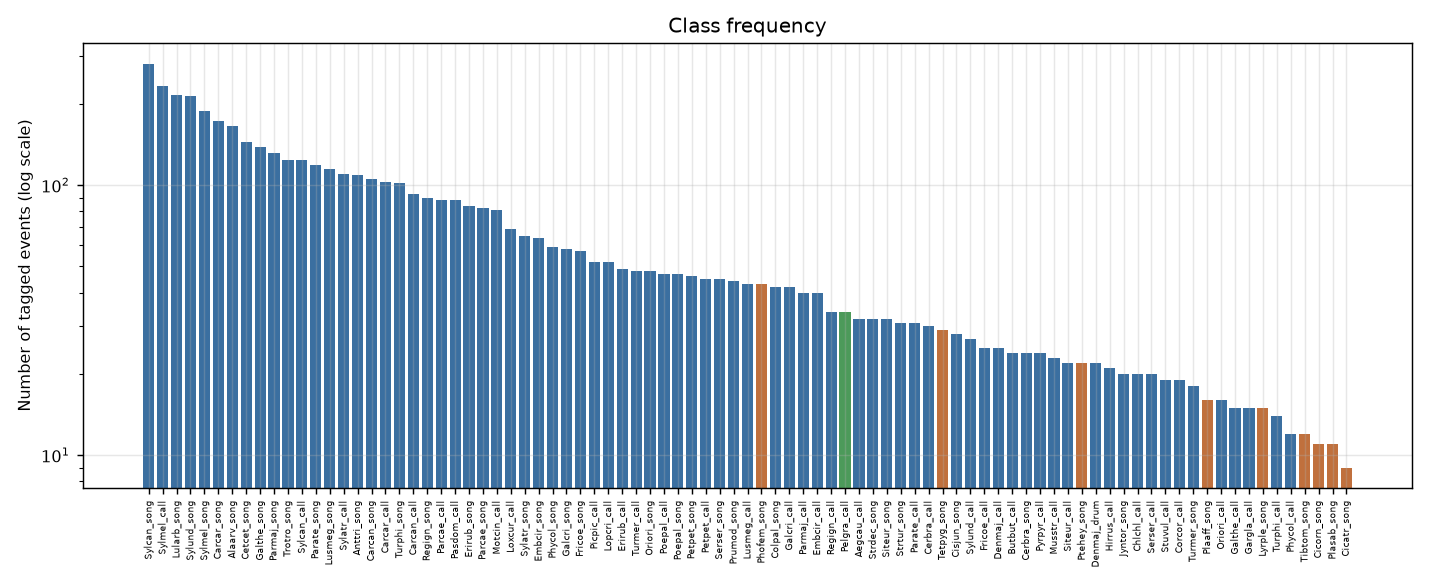
\includegraphics[width=0.72\textwidth]{figures/05_class_frequency.png}
\caption{Number of tagged events per class, all 87 classes, sorted, log scale.}
\label{fig:classfreq}
\end{figure}

The amplitude side of the dataset is similarly lopsided. Working out per-file statistics such as RMS energy and crest factor (the ratio between the loudest single sample and the average loudness of the whole file) across all 687 training recordings and fitting the same five distribution families again picks out lognormal as by far the best fit for both, again by a wide AIC margin, and again with heavy skew (skewness around 22 for RMS energy, and around 9 for crest factor). Standard normality tests such as Shapiro-Wilk reject the normal distribution for essentially every amplitude and spectral feature checked, but with roughly 687 recordings to work with, this kind of test is powerful enough to reject normality for almost any real measurement that has even a small amount of skew, so the rejection on its own is not that informative. What is informative is the actual shape: a small number of recordings are wildly more impulsive than the rest (one file in particular has a crest factor over 150, an order of magnitude beyond the next most extreme recording in the set, which visually turns out to be one sharp, loud call sitting inside an otherwise near-silent clip), and this means that a plain mean-and-standard-deviation summary of amplitude in this dataset is genuinely misleading, since it is being pulled around by a handful of outlier files.

Class imbalance is also worth putting a real number on rather than just calling it ``unbalanced''. Across the full 87-class scheme, the least represented class has 9 tagged events and the most represented class has 282, a 31.3 times gap between the two, and computing the Gini coefficient over the full class-count distribution gives 0.447, with an entropy of about 5.97 bits, which corresponds to an ``effective'' number of classes of roughly 62.5 out of the 87 that actually exist. Ranking classes by frequency and plotting on a log-log scale gives something close to a straight line with a slope near $-0.84$ ($R^2 \approx 0.88$), meaning class frequency in this dataset behaves roughly like a Zipf distribution, sitting somewhere between perfectly uniform and the kind of extremely long-tailed imbalance seen in some citizen-science bioacoustic datasets, where the gap between the most and least common class can run into the hundreds or thousands.

\begin{figure}[h]
\centering
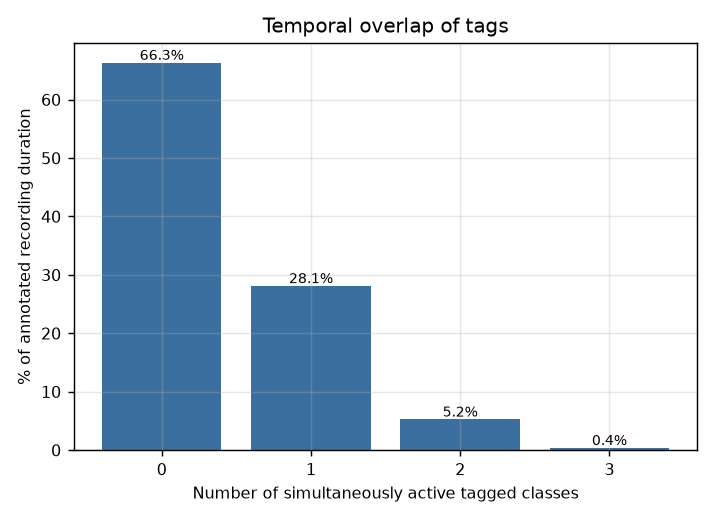
\includegraphics[width=0.72\textwidth]{figures/09_simultaneity.png}
\caption{How many tagged calls are active at the same instant, computed with a sweep-line over every annotation file's timeline. This reproduces \citet{morfi2019}'s own reported figures for the same statistic almost exactly (66.3/28.1/5.2/0.4 percent there, against 66.32/28.09/5.24/0.36 percent computed independently here).}
\label{fig:simultaneity}
\end{figure}

Finally, the overlap claim discussed again in Section 1.5 can be checked with a sweep-line over every file's set of tagged intervals (Figure~\ref{fig:simultaneity}), which shows that two-thirds of annotated time has no tag active, just over a quarter has exactly one tag active, and the remainder has two or more tags overlapping. At the level of individual events rather than time, 27.4 percent of the 5{,}775 tagged rows overlap in time with at least one other tagged row, and 24.0 percent overlap with a row carrying a \emph{different} label, which is a close, independent match to the paper's own ``over 20 percent'' claim, worked out here from the raw timestamps instead of from a review of predictions.

\subsection{What ``correct'' means here: the evaluation metrics}

Section 1.2 defines what the model outputs, but a full statement of the problem also needs to say what counts as getting the right answer, since accuracy alone can be a misleading number on an imbalanced, 87-class problem like this one. The paper reports six figures side by side for every run: accuracy, ROC-AUC, precision, recall, and top-3 and top-5 accuracy, all computed with weighted averaging across classes so that the rarer classes are not simply drowned out by the common ones. Weighted precision and weighted recall are computed as

\begin{equation}
\text{Precision} = \sum_{c=1}^{K} \frac{n_c}{N} \cdot \frac{TP_c}{TP_c + FP_c}, \qquad
\text{Recall} = \sum_{c=1}^{K} \frac{n_c}{N} \cdot \frac{TP_c}{TP_c + FN_c},
\end{equation}

where $n_c$ is the number of true examples of class $c$ and $N$ is the total number of test events. It is worth actually working through what weighted recall reduces to in a single-label, multi-class setting like this one, because it explains something that otherwise looks odd in the paper's own results table. Since every true instance of class $c$ is either correctly predicted ($TP_c$) or incorrectly predicted as something else ($FN_c$), the denominator $TP_c + FN_c$ is always exactly $n_c$, so

\begin{equation}
\text{Recall} = \sum_{c=1}^{K} \frac{n_c}{N} \cdot \frac{TP_c}{n_c} = \frac{1}{N}\sum_{c=1}^{K} TP_c = \frac{\text{total correct}}{N} = \text{Accuracy}.
\end{equation}

Weighted recall and accuracy are, algebraically, the same number in this setup, and that is exactly why the paper's own results table shows identical accuracy and recall figures on every single row, which could otherwise look like a copy-paste mistake at first glance.

Top-$k$ accuracy relaxes the strict argmax rule and instead asks whether the correct class is anywhere among the model's $k$ highest scoring guesses, which is a reasonable thing to report on a task with dozens of classes and meaningful label noise, since it separates ``the model was completely wrong'' from ``the model was close, and the right answer was its second or third guess''. The gap the paper reports between top-1 and top-3/top-5 accuracy on every class set is fairly large, which on its own is a hint that a meaningful share of the model's mistakes are near misses rather than wild guesses.

One thing worth flagging honestly here, since the assignment specifically asks for a critique of the metrics and not just a restatement of them: the way the model is actually scored at test time does not fully match what Section 1.2 describes. Section 1.2's per-event averaging rule implies that only frames belonging to the tagged event are ever scored, but the validation code in the released repository instead slides a frame across the \emph{entire} recording the tagged event came from, sums the log-probabilities from every one of those frames (most of which do not overlap the tagged call at all), and only then applies the argmax. On a five second recording where the tagged call itself might only last a tenth of a second, this means the vast majority of the frames being summed have nothing to do with the label being checked against, so the reported accuracy is, strictly, an answer to a slightly different and arguably easier question than ``can this model recognise this call'', namely ``does the overall content of this five second recording, background noise and all, still point the summed score toward the right class''.

\subsection{A formulation issue the authors acknowledge but do not resolve}

A serious issue is acknowledged by the paper but not properly resolved. In the NIPS4Bplus dataset, over 20 percent of the tagged sound events overlap with a sound from a different species \citep{bravosanchez2021}. In recordings, it is common for two or more birds to call simultaneously. Even though the task is formulated as single label multi class classification, it is more of a multi label classification problem, or a single label classification problem with label noise. The authors identified that, when a frame contains two overlapping calls, the model predicts a genuinely present species, even though that is not the recorded label, and re-scoring such cases as correct would push the headline accuracy up by around four points \citep{bravosanchez2021}. Section 1.3 above works out this same overlap statistic directly from the raw annotation timestamps rather than from a review of model predictions, and lands on a very similar number (27.4 percent of tagged events overlap something, 24.0 percent overlap a different label), which is a second, independent way of arriving at the same conclusion: a meaningful share of this dataset's ``ground truth'' is genuinely ambiguous, not just noisy in the ordinary sense.

\subsection{A second, unacknowledged formulation issue: how the split is drawn}

There is a second issue with how this problem is set up that the paper's discussion section does raise in passing but does not fully spell out the consequences of, and it concerns how the 75:25 train/test split described in Section 3.6 actually interacts with the way events are grouped. Because the split is drawn over individual tagged events rather than over whole source recordings, it is entirely possible, and in fact very common in this dataset, for one tagged event from a given five-second recording to land in the training list while a different tagged event from that exact same recording lands in the test list. Checking this directly against the class-set list files bundled with this project shows that, for the bird-classes scheme, 96.5 percent of the recordings that contribute to the test list also contribute a different tagged row to the training list. This means the model is very rarely being asked to generalise to a genuinely unseen recording at test time, since the background noise, the recording location's acoustic signature, and often other overlapping calls in that same clip were already available to it during training under a different label. The paper's own discussion section does acknowledge, citing prior work, that drawing training and test data from the same underlying pool is known to make a task easier than testing on an independently collected dataset \citep{xie2020}, but it frames this mainly as a general limitation of the field rather than something specific and measurable about its own particular 75:25 split, which the number above suggests it very much is.

\section{Methodological Justification}

\subsection{Why SincNet was chosen over a standard CNN on the raw waveform}

This paper uses SincNet \cite{ravanelli2018} instead of using a convolutional neural network directly on the raw waveform. This is because, according to prior work, feeding raw audio straight into an ordinary CNN puts heavy strain on that network's very first layer. This is due to the layer having to learn every individual filter coefficient from nothing, given how high dimensional a raw waveform chunk is, and this is known for introducing the vanishing gradient problem and requiring a large amount of labelled data \cite{bravosanchez2021}, citing \cite{ravanelli2018}.

To fix this, SincNet forces each filter into the shape of a band pass filter built from the sinc function, with only its lower and upper cutoff frequencies, $f_l$ and $f_h$, left as learnable numbers:

\begin{equation}
g[n, f_l, f_h] = 2f_h\,\mathrm{sinc}(2\pi f_h n) - 2f_l\,\mathrm{sinc}(2\pi f_l n), \qquad \mathrm{sinc}(x) = \frac{\sin(x)}{x},
\end{equation}

with $f_l, f_h \in \left[0, \dfrac{f_s}{2}\right]$ and $f_s$ the sampling frequency \citep[Eq.~2]{bravosanchez2021}. Due to this implementation, it takes the first layer's parameter count from 20,080 to 160, for the default 80-filter configuration used on the speech task this architecture was originally built for. The same trade works out even more dramatically for the tuned bioacoustic configuration described in Section 2.3, which uses 220 filters of length 151: an ordinary convolution of that size would need $220 \times 151 = 33{,}220$ separate numbers in its first layer, while the sinc-constrained version needs only $220 \times 2 = 440$, a roughly 75-fold reduction in exactly the layer that would otherwise be the hungriest for data.

\begin{figure}[h]
\centering
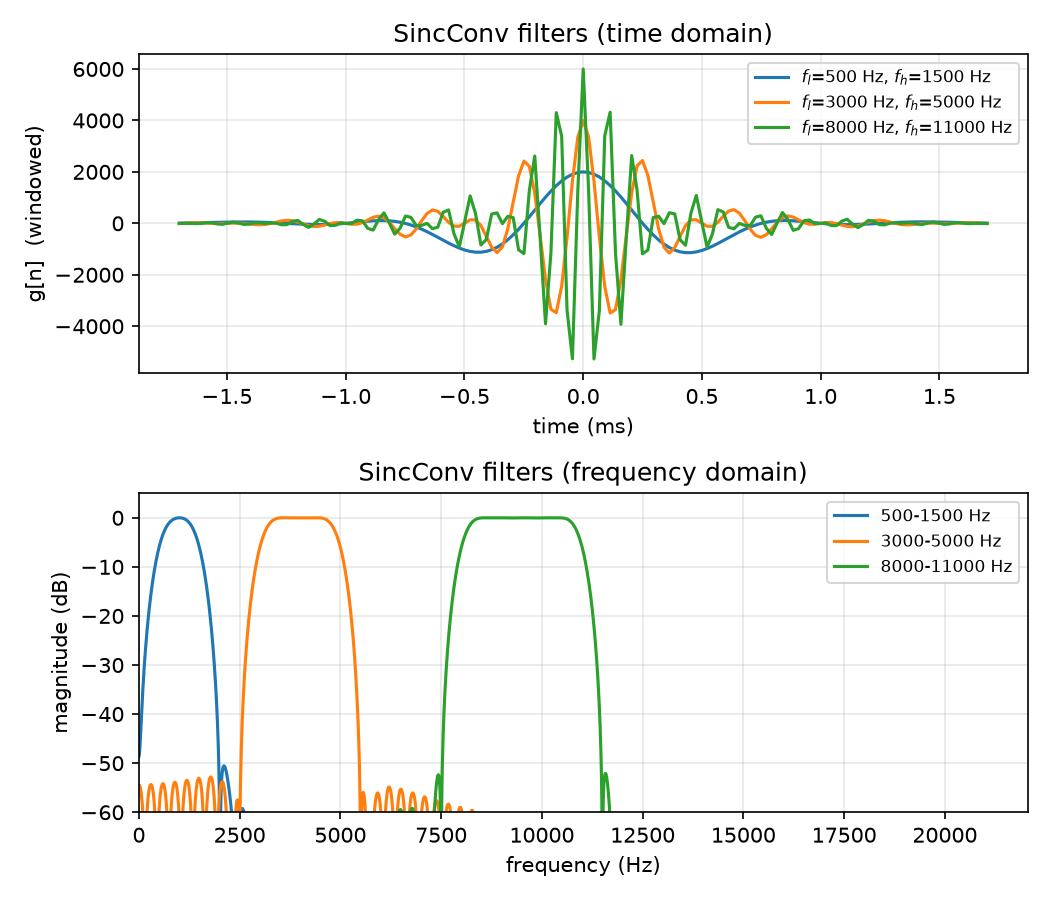
\includegraphics[width=0.78\textwidth]{figures/16_sincconv_filter_response.png}
\caption{Three example SincNet filters, computed directly from the equation above at the filter length used in the tuned configuration ($L=151$). Top: the filter itself in the time domain, after the Hamming window is applied. Bottom: the same filter's frequency response, which approximates a rectangular pass-band between $f_l$ and $f_h$.}
\label{fig:sincfilters}
\end{figure}

This gains efficiency by shrinking the hypothesis space. A CNN searches all the possible length $L$ filter vectors. Even though this space contains every band pass filter, it also contains shapes that are not useful for this task at all. Instead, SincNet only searches inside a two dimensional family of band pass filters. This is because the filters that are most relevant for the audio task are more likely to be similar to a band pass filter. This technique narrows the search surface without sacrificing much of the performance. The authors describe the constraint as one that ``converges faster and performs better than a standard CNN'' while needing less training data \citep{bravosanchez2021}.

It is worth adding two smaller design details that sit underneath this same first layer, since they help explain why it behaves the way it does rather than just how it is built. First, the filters are not started from a random position; they are initialised using the Mel scale, which spaces the starting cutoffs more densely at lower frequencies, on the reasoning that lower frequencies tend to carry more perceptually relevant structure. But the paper itself also notes, somewhat surprisingly, that once training is finished the filters have not actually moved very far from where the Mel scale placed them, which suggests this first layer is behaving more like a carefully chosen fixed filterbank with light fine-tuning than like a fully free filter search, despite being described as ``learned''. Second, since the sampling rate here is 44.1~kHz rather than the 16~kHz used in the original speech task, the learnable upper cutoff $f_h$ is bounded at 22.05~kHz (half the sampling rate, by the Nyquist limit), and this higher ceiling is itself one of the practical reasons the higher sampling rate matters: a lower sampling rate would make a real chunk of the birds' and especially the insects' acoustic range simply unreachable by this filterbank, regardless of how the rest of the architecture is tuned.

\subsection{Why the comparison models were chosen}

In order to evaluate each part of the model, researchers constructed two categories of comparison models. The first one is called ``waveform + CNN''. It uses the same architecture as SincNet, but replaces the first sinc based convolution with a normal convolutional layer \citep{bravosanchez2021}. This is used to test the specific contribution of the sinc based convolution.

The second one is transfer learning on three pretrained ImageNet backbones, namely DenseNet121, ResNet50, and VGG16, fine tuned on image representations of the audio (for example, spectrograms, Mel spectra, and MFCCs) instead of the raw waveform \citep{bravosanchez2021}. This is the paradigm that was established before this research, and it is used to evaluate how SincNet performs against other, more established methodologies.

\subsection{Why the TIMIT hyperparameters were largely retained}

This research paper initially keeps the SincNet hyperparameters at the defaults used in the original TIMIT speaker recognition experiment \citep{ravanelli2018}, instead of tuning them to maximise performance in the bioacoustic domain. According to the authors, they did this in order to ensure the easy reproducibility of their results. If tuned to maximise performance, it would be more difficult to reproduce due to undisclosed tuning decisions \citep{bravosanchez2021}.

In the second stage, they use grid search on window size, filter counts, normalisation type, and other parameters to obtain an enhanced, tuned SincNet result for comparison against the other models \citep{bravosanchez2021}.

This is a great decision by SincNet's authors. Instead of presenting the most impressive numbers, they divided their methodology to ensure easy and reliable reproduction. It also showcases that SincNet has high domain transferability, where it performs well even though the hyperparameters are tuned for a different task. This suggests that SincNet can be dropped onto a new domain without specific tuning and still produce a reasonable result.

\subsection{The training workflow, one layer at a time}

The two subsections above explain \emph{why} SincNet was picked and why the hyperparameter strategy was split into a default stage and a tuned stage, but they do not really walk through what actually happens to a frame once it enters the network, and the assignment specifically asks for that level of detail, so Figure~\ref{fig:workflow} lays out the full path from a raw frame to a training update, and the paragraphs after it go through each stage and try to justify it on its own terms, including saying plainly where a normalisation layer, an activation function, or a dropout rate is or is not being used, since that is easy to get wrong just from reading the paper's prose alone.

\begin{figure}[h]
\centering
\resizebox{0.92\textwidth}{!}{%
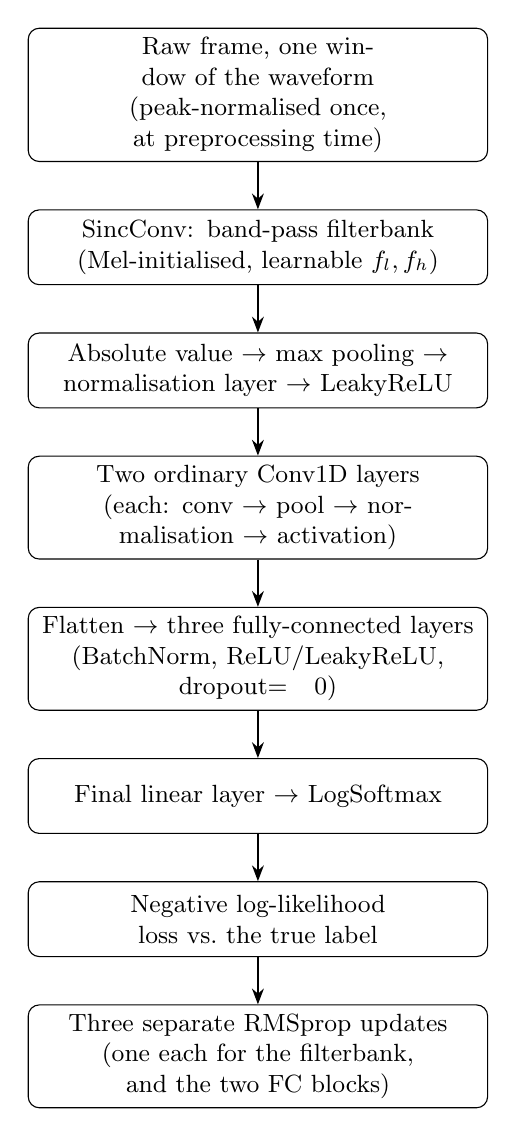
\begin{tikzpicture}[
  node distance=6mm and 6mm,
  box/.style={rectangle, draw, rounded corners, align=center, text width=5.6cm, minimum height=0.95cm, font=\small},
  arr/.style={-{Stealth[length=2mm]}, thick}
]
\node[box] (a) {Raw frame, one window of the waveform\\(peak-normalised once, at preprocessing time)};
\node[box, below=of a] (b) {SincConv: band-pass filterbank\\(Mel-initialised, learnable $f_l,f_h$)};
\node[box, below=of b] (c) {Absolute value $\to$ max pooling $\to$\\normalisation layer $\to$ LeakyReLU};
\node[box, below=of c] (d) {Two ordinary Conv1D layers\\(each: conv $\to$ pool $\to$ normalisation $\to$ activation)};
\node[box, below=of d] (e) {Flatten $\to$ three fully-connected layers\\(BatchNorm, ReLU/LeakyReLU, dropout$=0$)};
\node[box, below=of e] (f) {Final linear layer $\to$ LogSoftmax};
\node[box, below=of f] (g) {Negative log-likelihood loss vs.\ the true label};
\node[box, below=of g] (h) {Three separate RMSprop updates\\(one each for the filterbank, and the two FC blocks)};
\draw[arr] (a)--(b); \draw[arr] (b)--(c); \draw[arr] (c)--(d);
\draw[arr] (d)--(e); \draw[arr] (e)--(f); \draw[arr] (f)--(g); \draw[arr] (g)--(h);
\end{tikzpicture}}
\caption{The training path a single frame follows, from raw samples to a gradient update, as it is actually implemented in the released training script.}
\label{fig:workflow}
\end{figure}

\paragraph{Normalisation before the model even sees the data.} The only scaling step applied anywhere in the pipeline is a per-file peak normalisation, where every sample in a recording is divided by that recording's own largest value, so that every file's loudest sample sits at exactly 1.0. This is a reasonable thing to want, since two recordings of the same bird at different distances can otherwise have very different absolute loudness for no reason related to species identity. But given what Section 1.3 found about RMS energy and crest factor both being lognormally distributed, with a small number of files behaving like extreme outliers, dividing by a single largest sample is a slightly fragile choice of scaling statistic, since it is set entirely by one sample in the whole file rather than by anything closer to the file's typical loudness, such as its RMS energy. The implementation used in the released code also divides by the largest \emph{signed} value rather than the largest \emph{magnitude}, which means that whenever a file's biggest swing happens to be a negative excursion, the ``normalised'' file can actually end up slightly louder than the 1.0 ceiling this step is supposed to guarantee. This is left as an observation rather than something worth changing, since it is the authors' own released preprocessing and presumably is baked into their own reported numbers as well.

\paragraph{Is batch normalisation used? Yes, in most of the network, but not consistently.} Checking the actual configuration files that ship with the tuned runs directly answers this rather than guessing at it from the paper's prose: batch normalisation is switched on for all three fully-connected layers in both the default and the tuned configuration, and it is also switched on for all three convolutional layers in the tuned configuration specifically. The earlier, default configuration instead uses layer normalisation on its convolutional layers rather than batch normalisation. Batch normalisation rescales each layer's activations using the mean and variance of the current minibatch, which tends to let training tolerate a higher learning rate and converge faster, and the fact that it is used so widely here, on a network that otherwise has zero dropout anywhere (see below), is probably doing a meaningful share of whatever regularisation this network gets. Layer normalisation, used instead on the earlier convolutional layers, normalises across a single example's own features rather than across the batch, which is a more robust choice when batch statistics might not be reliable, though nothing in the paper's text explains why the switch from layer normalisation to batch normalisation was made when moving from the default to the tuned configuration; it reads more like a choice that came out of the grid search mentioned in Section 2.3 than a decision made for a bioacoustic-specific reason.

\paragraph{Is dropout used? No, not anywhere, in either configuration.} Every dropout setting in every configuration file bundled with this project, for the convolutional layers, the fully connected layers, and the final classification layer alike, is set to exactly 0.0. This is worth stating plainly, because the paper's text does say dropout was one of the parameters swept during the grid search stage, which could give the impression that some non-zero dropout rate made it into the final tuned model; the tracked configuration files say otherwise. Given a training pool of under 4,000 tagged events feeding into fully-connected layers with over a thousand units each, and given the class imbalance already measured in Section 1.3, a network with this much capacity and zero dropout is a fairly classic setup for overfitting, and this lines up with what was actually observed when this pipeline was run in this project: training error kept dropping well past the point where test error had already flattened out.

\paragraph{The output layer and the loss function.} The configuration files describe the final activation as ``softmax'', but the model implementation actually applies LogSoftmax and pairs it with a negative log-likelihood loss, which is not really a discrepancy once worked through mathematically: for a target class $y$ and log-probabilities $\log \hat p$, $-\log \hat p_y$ is exactly the standard cross-entropy loss evaluated on a one-hot target, just computed in a more numerically stable order that avoids taking a separate logarithm of a potentially tiny softmax output. So the configuration field name is a slightly misleading label for what is, underneath, an entirely standard and correct classification loss.

\paragraph{The optimiser.} Training uses RMSprop, with a separate optimiser instance for the filterbank and for each of the two fully-connected blocks, all sharing the same learning rate of 0.001 and the same smoothing constant $\alpha = 0.95$. RMSprop keeps a running average of each parameter's squared gradient and divides the update by its square root, which lets parameters with very different natural scales, such as the filterbank's cutoff frequencies (which live on a scale of thousands of Hz) against the fully-connected layers' ordinary small weights, each get a step size suited to their own scale, without needing the learning rate to be hand-tuned separately for each part of the network. Using three separate optimiser objects rather than one combined optimiser does not actually change this maths, since each parameter still keeps its own running average regardless of which object it is attached to; it looks more like a code organisation choice than a distinct optimisation strategy. There is no learning rate schedule anywhere in the training script either, the learning rate is held constant for the entire run, which is a defensible simplification given RMSprop's own adaptive behaviour, but a fixed or step decay schedule would have been a fairly low-risk addition on top of it.

\subsection{Hyperparameter strategy, data splitting, and model selection, examined more critically}

Section 2.3 already covers, in general terms, why the paper splits its hyperparameter search into a default stage and a tuned stage, but it is worth looking a bit more carefully at how the ``best'' configuration is actually chosen once the grid search is run, since this has a real statistical consequence. The paper describes repeating the training sequence across five different random train/test splits and reporting the model that performs best; but there does not appear to be a separate validation set distinct from the test set that gets reported as the final number, only a training list and a test list. Repeatedly trying different hyperparameter settings and reporting whichever one scores highest against the same held-out set that then becomes the headline number is a well known way to end up with an optimistic estimate, since the winning configuration is, to some extent, being selected \emph{for} performing well on that particular test split rather than being an unbiased read on how it would do on genuinely new data. This is a very common situation for a paper working with a dataset this small to end up in, and the authors are upfront about the multi-run methodology, but it is a real soft spot in the model-selection process worth naming directly rather than glossing over.

It is also worth being precise about how many training steps ``one epoch'' actually represents in this codebase, since the tuned configuration and the default configuration are not directly comparable on epoch count alone. Because minibatches are drawn by uniformly sampling tagged events with replacement rather than by looping over a fixed training set, the true unit of training budget is the number of minibatches times the number of epochs, not the epoch count on its own. The default configuration runs 200 epochs of 800 batches each, for 160{,}000 total gradient steps, while the tuned configuration runs 400 epochs of only 80 batches each, for just 32{,}000 total gradient steps, five times fewer. So on paper the tuned model looks like it trains for twice as long, but in terms of how many times its weights are actually updated, it trains for a fifth as long, and comparing the two configurations by epoch count without accounting for this would be a straightforward mistake.

\section{Data Pipeline Analysis}

\subsection{Source, format, and provenance of the raw data}

This research uses the NIPS4Bplus dataset for training. It is a dataset built on top of the 2013 Neural Information Processing Scaled for Bioacoustics (NIPS4B) bird song classification challenge \cite{glotin2013}, as cited in \cite{bravosanchez2021}. The dataset consists of 687 short field recordings from central and southern France and southern Spain, where each recording is one to five seconds long. They are captured on a single channel at 44.1 kHz with 32 bit depth \cite{bravosanchez2021}. When the dataset first came out, it only had labels that stated a species was present somewhere in a file, but not when. To fix this problem, \citet{morfi2019} re-annotated the dataset with precise start times and durations for every individual vocalisation by hand, using an experienced ornithologist and dedicated software, and it is this re-annotated version that is used in this research.

It is worth noting one small factual wrinkle that only becomes visible once the actual audio files are read rather than just trusting the metadata: every one of the 687 files, checked directly with an audio library for this assignment, reports a bit depth of 16-bit PCM rather than the 32-bit depth quoted above and stated in the paper's own text. This does not affect anything downstream, since every script that reads these files immediately decodes them into floating point before doing anything else with them, but it is a genuine mismatch between what the paper says about the release and what the released files themselves actually contain.

\subsection{Preprocessing steps applied by the authors}

For preprocessing, the authors used a Python script to take each individually tagged sound event from its parent recording, store it in a standalone waveform file, and apply amplitude normalisation. This is similar to what is done in normal speech recognition pipelines, such as trimming quiet stretches from the front and back of a recording before training \citep{bravosanchez2021}. In preprocessing, three recordings under 10 ms in length are also excluded from the training set.

To ensure proper usability in the new domain, some of the original TIMIT speech settings had to be adjusted. For example, the window frame size, the \texttt{cw\_len} setting, dropped from 200 ms to 10 ms. This is due to the fact that most bird sounds in the dataset last only a few milliseconds. With that change, the window shift, \texttt{cw\_shift}, also dropped from 10 ms to 1 ms. To match what NIPS4Bplus uses, the sampling frequency was also increased from 16,000 Hz to 44,100 Hz. Depending on the run, the final layer's class count, \texttt{class\_lay}, was swapped due to different label granularities of 87, 77, or 51. In later runs, the authors also replaced the simple file cropping approach with a more advanced approach, which reads the original, uncropped files and selects the labelled call directly from them, and uses padding when a call is shorter than the window frame \citep{bravosanchez2021}, following the two-branch rule already worked through in Section 1.2.

\subsection{Missing values, or the closest thing this pipeline has to them}

This dataset does not have missing values in the usual tabular sense, an empty cell in a spreadsheet, but it does have a close structural equivalent that the pipeline handles in a way worth spelling out, since the assignment specifically asks how missing values are handled and simply saying ``there are none'' would be missing the point. An annotation record for a given recording can be in one of three states: present with at least one tagged row (the normal case, 569 of the 687 files), present but genuinely empty, meaning a reviewer looked at the recording and found nothing worth tagging (105 files), or entirely absent, meaning no annotation record exists for that file at all (13 files). The preprocessing scripts treat the second and third cases identically: both simply contribute zero rows to the final training list, with no imputation and no special ``unknown'' label standing in for the missing information. But these two cases are not actually the same thing epistemically. An empty-but-present record is a confirmed negative, a person deliberately decided there was nothing there, while an absent record is a genuine unknown, nobody ever made that call either way. Collapsing both into ``this file contributes nothing'' loses that distinction, and any later analysis that checks ``does this file have any tagged events'' without separating the two would silently misclassify the provenance of well over a hundred files.

\subsection{Feature scaling, or the lack of it}

Because the input to this model is the raw waveform itself rather than a table of hand-built features, there is no per-feature scaling step in the usual machine learning sense, no z-scoring or min-max scaling being applied to a design matrix, since there is no design matrix to begin with. The only scaling that happens anywhere is the peak amplitude normalisation described in Section 2.4, applied once per file during preprocessing, plus a small multiplicative jitter (multiplying the windowed frame by a random number drawn between 0.8 and 1.2) applied fresh every time a frame is drawn during training. As already argued in Section 2.4, given that RMS energy and crest factor were both found to be lognormally distributed with heavy skew in Section 1.3, a scaling statistic built from the single loudest sample in a file is a somewhat fragile choice, and a scaling statistic built from something closer to the file's typical energy, such as its RMS value, or a log-compressive transform, would sit more naturally with the actual measured shape of the amplitude distribution, though this is offered here as an observation about the statistical fit of the method rather than a claim that the released preprocessing is wrong.

\subsection{Non-handling of class imbalance}

Due to this dataset being a set of audio taken from the wild, the dataset is highly unbalanced. As an example, there are only 9 black cicada songs, while there are 282 subalpine warbler calls \citep{bravosanchez2021}, a gap that Section 1.3 above puts a formal number on: a 31.3-times ratio between the rarest and most common class, a Gini coefficient of 0.447 over the full 87-class distribution, and a class-frequency curve that behaves roughly like a Zipf distribution. Even though the dataset is unbalanced, this research paper does not describe any balancing interventions to fix this issue, and neither does the released training code: minibatches are built by drawing tagged events completely uniformly at random, with no weighting by inverse class frequency, and the loss function itself is not given any per-class weights either. This means a class with 282 examples is roughly 30 times more likely to show up in any given minibatch than a class with 9 examples, so whatever imbalance exists in the raw dataset is passed straight through into how often the model's weights get updated in response to each class, completely unmodified. Due to this class imbalance, confusion matrix analysis shows that the model's predictions skew towards the best represented sound classes in the training data, while some underrepresented sound classes do not receive correct predictions \citep{bravosanchez2021}.

\subsection{Train and test split methodology}

To divide the dataset into train and test sets, the research uses another custom Python script. That script randomly assigns files into training and test lists at a 3:1 ratio, using a dictionary that maps each file to its class \citep{bravosanchez2021}. They do this split after taking the cropped events, instead of splitting the original recordings, which is exactly the issue quantified in Section 1.6 above (96.5 percent of test-list recordings, for the bird-classes scheme, also contribute a different event to the training list). The authors cite \citet{xie2020}, acknowledging that taking training and testing samples from the same dataset makes a classification task easier than using an independent, different dataset. This means that, in the real world, performance might be lower in different locations, fields, and equipment. The researchers also repeat the entire training sequence across five different train and test splits, to ensure that the performance metrics are valid.

One more detail worth adding here, since it only becomes visible once the actual split-generation script bundled with this project is read rather than just its description: the random split is drawn without a fixed random seed, meaning every time the split-generation script is re-run it produces a genuinely different training and test list, and, because the class labels themselves are assigned as plain integers based on the order classes first appear in that particular run's file list, a different run also assigns a different integer to the same species. A model checkpoint trained against one run of this script is therefore not meaningfully evaluable against a freshly regenerated list from a later run, since class index 7, say, might mean one species under the old list and a completely different species under the new one. This is a genuine reproducibility gap sitting underneath the split methodology, separate from the leakage issue above, and it is the kind of thing that only shows up once someone actually tries to re-run the released pipeline rather than just reading about it.

\subsection{The pipeline end to end, and where it could reasonably be improved}

Pulling the last four subsections together into one picture, Figure~\ref{fig:pipeline} lays out the full path from the raw recordings on disk to a trained model's reported metrics, and marks, at each stage, roughly where the issues raised above actually sit.

\begin{figure}[h]
\centering
\resizebox{0.95\textwidth}{!}{%
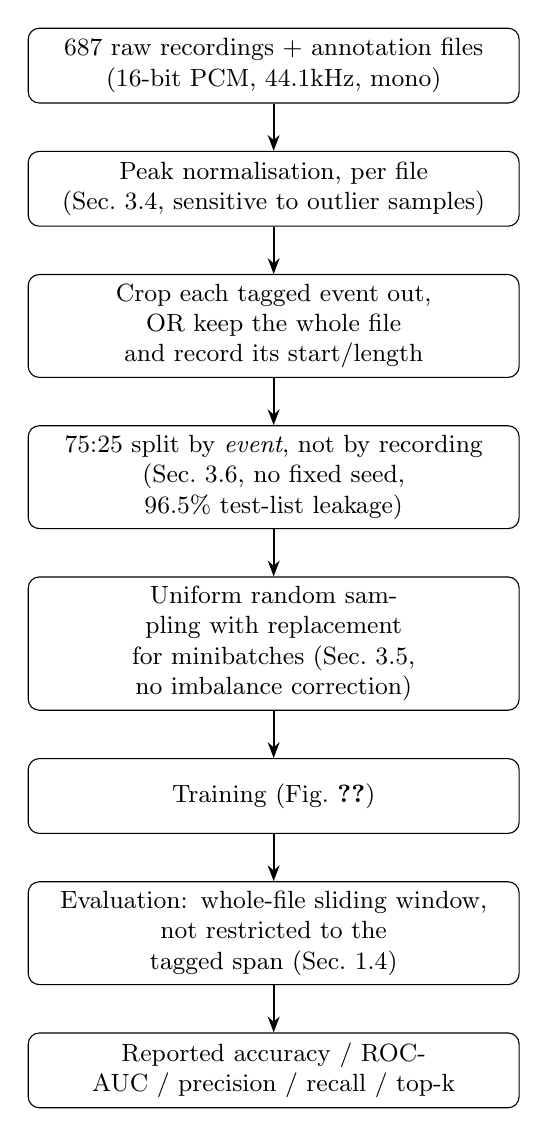
\begin{tikzpicture}[
  node distance=6mm and 6mm,
  box/.style={rectangle, draw, rounded corners, align=center, text width=6.0cm, minimum height=0.95cm, font=\small},
  arr/.style={-{Stealth[length=2mm]}, thick}
]
\node[box] (a) {687 raw recordings + annotation files\\(16-bit PCM, 44.1kHz, mono)};
\node[box, below=of a] (b) {Peak normalisation, per file\\(Sec.~3.4, sensitive to outlier samples)};
\node[box, below=of b] (c) {Crop each tagged event out,\\OR keep the whole file and record its start/length};
\node[box, below=of c] (d) {75:25 split by \emph{event}, not by recording\\(Sec.~3.6, no fixed seed, 96.5\% test-list leakage)};
\node[box, below=of d] (e) {Uniform random sampling with replacement\\for minibatches (Sec.~3.5, no imbalance correction)};
\node[box, below=of e] (f) {Training (Fig.~\ref{fig:workflow})};
\node[box, below=of f] (g) {Evaluation: whole-file sliding window,\\not restricted to the tagged span (Sec.~1.4)};
\node[box, below=of g] (h) {Reported accuracy / ROC-AUC / precision / recall / top-k};
\draw[arr] (a)--(b); \draw[arr] (b)--(c); \draw[arr] (c)--(d);
\draw[arr] (d)--(e); \draw[arr] (e)--(f); \draw[arr] (f)--(g); \draw[arr] (g)--(h);
\end{tikzpicture}}
\caption{The full pipeline from raw files to reported metrics, with the main issues raised in Sections 1 and 3 marked at the stage they actually occur.}
\label{fig:pipeline}
\end{figure}

None of the individual choices in this pipeline are unreasonable on their own, each one has a genuine rationale behind it, peak normalisation genuinely does remove a real nuisance variable, stratified splitting genuinely does respect class imbalance, and so on, but a few of them compound in ways that are only visible once the pipeline is looked at end to end rather than one script at a time. If this pipeline were being rebuilt rather than reproduced, the two changes that would matter most, based on everything measured above, would be: splitting by source recording rather than by event, so that a file's audio cannot appear on both sides of the train/test boundary under two different labels; and giving the minibatch sampler some awareness of class frequency, whether through a weighted sampler or a weighted loss, so that the 31-times imbalance measured in Section 1.3 stops being passed straight through into training unmodified. A fixed random seed for the split-generation script would also be a small, low-risk fix for the reproducibility gap raised in Section 3.6, and would cost nothing in terms of how the model itself behaves. These are offered here as a description of what a more careful version of this pipeline could look like, not as a claim that the released code is broken; it clearly works well enough to train the models the paper reports.

\bibliography{references}

\section*{AI Acknowledgement}

Claude (developed by Anthropic) was used during the preparation of this document to assist with the exploratory statistical analysis of the raw dataset files described in Section~1.3, drafting the two pipeline diagrams (Figures~\ref{fig:workflow} and \ref{fig:pipeline}), and formatting the \LaTeX{} source code of this report. Overleaf was used as the environment in which this document was written and compiled.

\end{document}
